

\section{AVIST}
This section presents the design and implementation of AVIST. The core part of AVIST is a data dependency graph, which incorporated with multiple visualization and interaction techniques for charactering data transformations to highlight data aggregation on demand.  

%Coordinated and multiple views are provided in AVIST. Brushing and linking, animation and dynamic queries are deployed in data views. More importantly, AVIST features a data dependency graph for charactering data transformations, provides data aggregation and visual primitives generations together on demand.
 
\subsection{Visualization and Interaction}

%figure shows the design of the views. parallel 



Three data views are provided: histogram view, parallel coordinated view and dynamic view. More data views can be flexible added. For example, we add a virtual globe view for spatial data visualization in our case studies. Users can directly apply brushing and linking interaction on these views. 

\textbf{Histogram view} shows the data distribution of  current time window. Users can select different dimensions  from a listbox to explore different aggregation information.

\textbf{Parallel coordinate views} show  details of each data record in current window. Users can select multiple data dimensions to generate their custom parallel coordinate plots. The axes can be re-ordered based on users' selected order in the listbox.

\textbf{Dynamic view} is a time series  chart, which shows the data aggregation of certain filtered events over a period of time. When a user change data filters, the dynamic view clears previous results and re-draw everything. 

\textbf{Control panel} provides animation and dynamic query interactions.
%By playing the animation of the data at certain pace,  hidden temporal patterns can be revealed. 
The animation supports automatic forward playback, interactively dragging of the time window bar, and interactive change of animation speed. By changing the current time and time range, users can define a time window in which the information will be analyzed and visualized at the correlated views. By combining automated animation with these correlated views, AVIST provides  temporal changes in the datasets, which supports  discovery temporal patterns for further analysis.

\begin{figure}[htb]
	\centering
	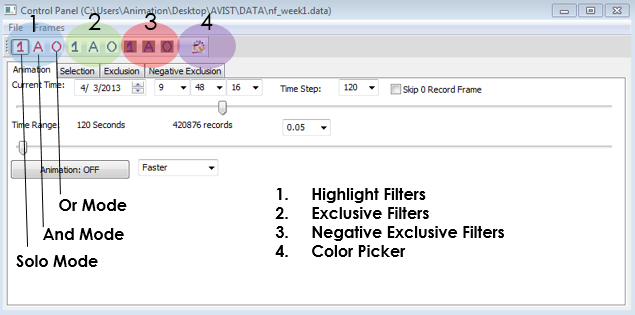
\includegraphics[width=1.0\linewidth]{pic/control.png}
	\parbox[t]{1.0\columnwidth}{\relax
	}
	%
	\caption{\label{fig:control} The control panel of AVIST. Three filters (\textit{highlight filter, exclusive filter and negative exclusive filter}) with three modes (\textit{solo mode, and mode, and or mode}) are provided. }
\end{figure} 

Besides animations, AVIST features the combined data filtering as shown in Figure~\ref{fig:control}. Three different filters are implemented: 1) highlight filters which make users' selected values stand out of the rest data with different colors,  2) exclusive filters to remove non-interesting data from data views and 3) negative exclusive filters, the exact opposite of exclusive filters, which remove all data except items marked interesting by a user. Each kind of data filters have three  modes: 1) \emph{Solo mode} , which allows only one filter value in current filter set, 2) \emph{and mode}  to combine several filters together as a complex filter emphasizing that data records need satisfy all requirements for visualization and 3) \emph{or mode}, which means that data records just need to meet only one of the filter requirements. 
Based on these three basic filters with their three modes, users can nest them to generate complex data filters which help to drill down each piece of data record. These filters with the brushing and linking interaction technique can quickly help users to explore datasets. 
%In Figure~\ref{fig:views}, users choose  highlight filters with \emph{or mode}, and then brush their selected colors in \textit{firstSeenDespIp} axis of parallel coordinated view to identify three suspicious IP addresses. The histogram view shows the distributions of \textit{ipLayerProtocol}, which emphasizes the highlighted activities in TCP flows. The dynamic view shows the highlighted records are a  periodically behavior in the network.

%for visual analysis large cyber security datasets, users can directly apply exclusive filter on port 80 to remove related network records to clear the visualization. After it, all three data views are immediately updated, and potential visual patterns may appear.


\subsection{Data Dependency Graph}

We character data transformations using a data dependency graph, which emphasizes data computation and visualization are on demand, triggered by user interactions. 

\begin{figure}[htb]
	\centering
	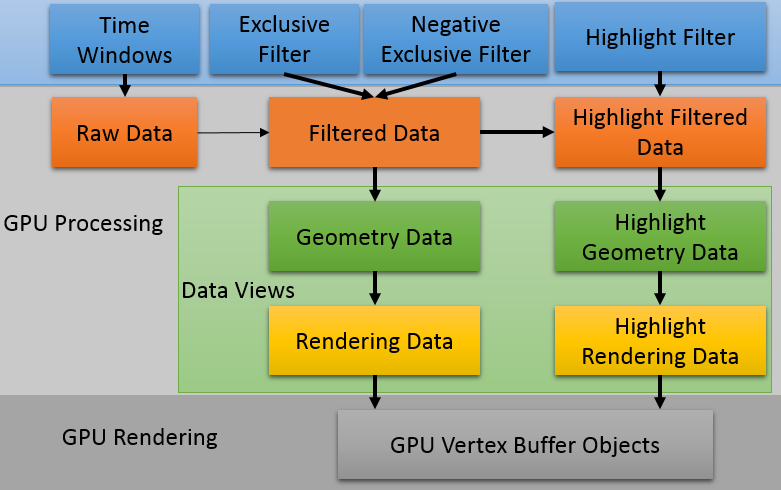
\includegraphics[width=1.0\linewidth]{pic/graph.png}
	\parbox[t]{1.0\columnwidth}{\relax
	}
	%
	\caption{\label{fig:datagraph} The data dependency graph of AVIST, which includes three layers: data filters, data processing and data rendering.}
\end{figure} 

% consider the cross filter design pattern 
%We employ the cross filtering design pattern \cite{weaver2010cross} in our GPU based in-situ visualization architecture, which contributes  a data dependency graph for organizing the data flow on the GPU.

Figure~\ref{fig:datagraph} shows our data dependency graph, which is separated into three parts. Firstly, the top level graph shows the user interactions in CPU side. Users can manipulate four filters generated by their interactions: \emph{time windows}, \emph{exclusive filter}, \emph{negative exclusive filter} and \emph{highlight filter}. All filters are passed into GPU  for data processing. The middle part of the graph is the GPU parallel processing. The raw data is filtered by \emph{time windows} first, then both \emph{exclusive filter} and \emph{negative exclusive filter} are applied to remove relevant data items. At last, \emph{highlight filter} is deployed to generate highlight datasets. Then, there are two steps to transform filtered data into visual primitives of each data view: 1) the geometry data is the aggregation of filtered data; 2) then rendering data follows, which transforms the aggregation data into visual primitives. At last, all rendering data are passed into GPU vertex buffer objects (VBOs). This kind of design makes that all data views share the raw data, filtered data and highlight filtered data, while each data view has its own geometry and rendering data. The last part in this graph is GPU rendering, which transforms all visual primitives into pixel colors.  




Our data dependency graph has several advantages. First, it follows the cross filtering design pattern~\cite{weaver2010cross} and three filters with three modes supports the drill down query of multi-dimensional datasets. 
%Users interactions trigger the data flows to update the visualizations. 
Second, all data processing and visual rendering can fully utilize GPU resources to achieve best performance with minimum IO costs. 
Third,  incremental computing can be applied to exploit temporal and spatial locality. When users play animation, frame-to-frame coherence can be exploited. In such cases, only incremental data need to be considered. Besides, user interactions also follow incremental format for dill-down queries. If a user perform \emph{or} operator of highlight filters, previous highlighting visual primitives do not need to be recomputed. When performing \emph{and} operator, incremental computing is only applied in previous highlight data which trigger the right column of data graph, while all other data are still the same. In all, we formalize the computation flow as a direct acyclic graph (DAG) of tasks, fully incorporated user interactions and incremental computing.

%one page
%// and or not similar with SQL  ad hoc visual query
%//multiple coordinate views space 
%//animation 	time

 
\subsection{Implementation}
AVIST is written in C++, its computation codes are based on CUDA 5.5 and visualization codes are based on OpenGL and GLSL. The interface are coded by wxWidgets. We use the Thrust library\footnote{https://developer.nvidia.com/Thrust} for accelerating sort, scan, transform and reduction operations.


\begin{figure}[htb]
	\centering
	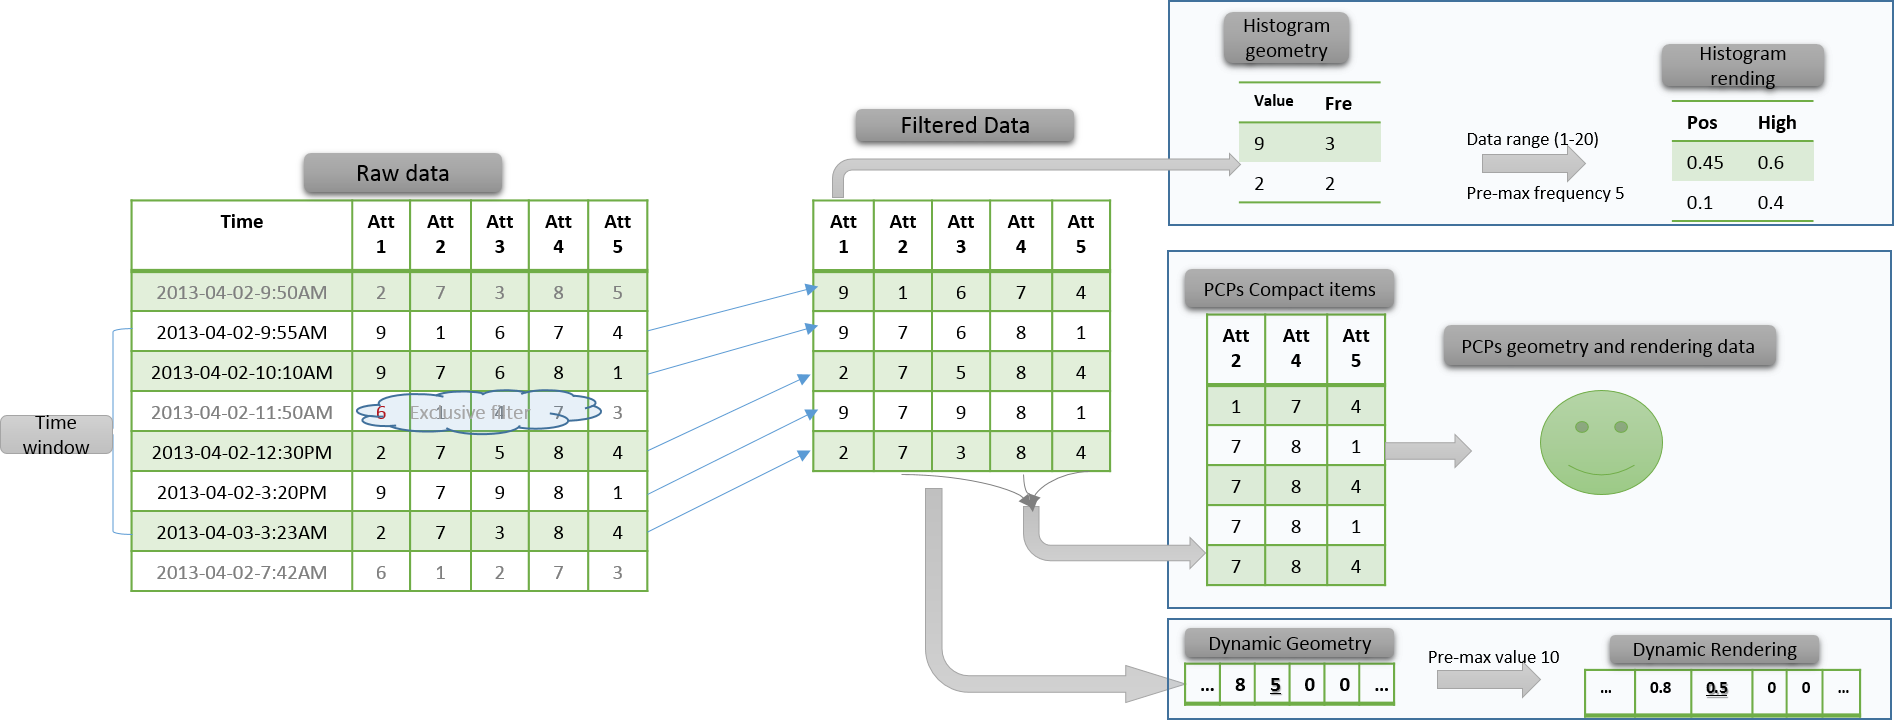
\includegraphics[width=1.0\linewidth]{pic/dataTran1.png}
	\parbox[t]{1.0\columnwidth}{\relax
	}
	%
	\caption{\label{fig:dataTran1} This figure shows data transformations from raw data to  geometry and rendering data of histogram and dynamic view.}
\end{figure} 

\begin{figure}[htb]
	\centering
	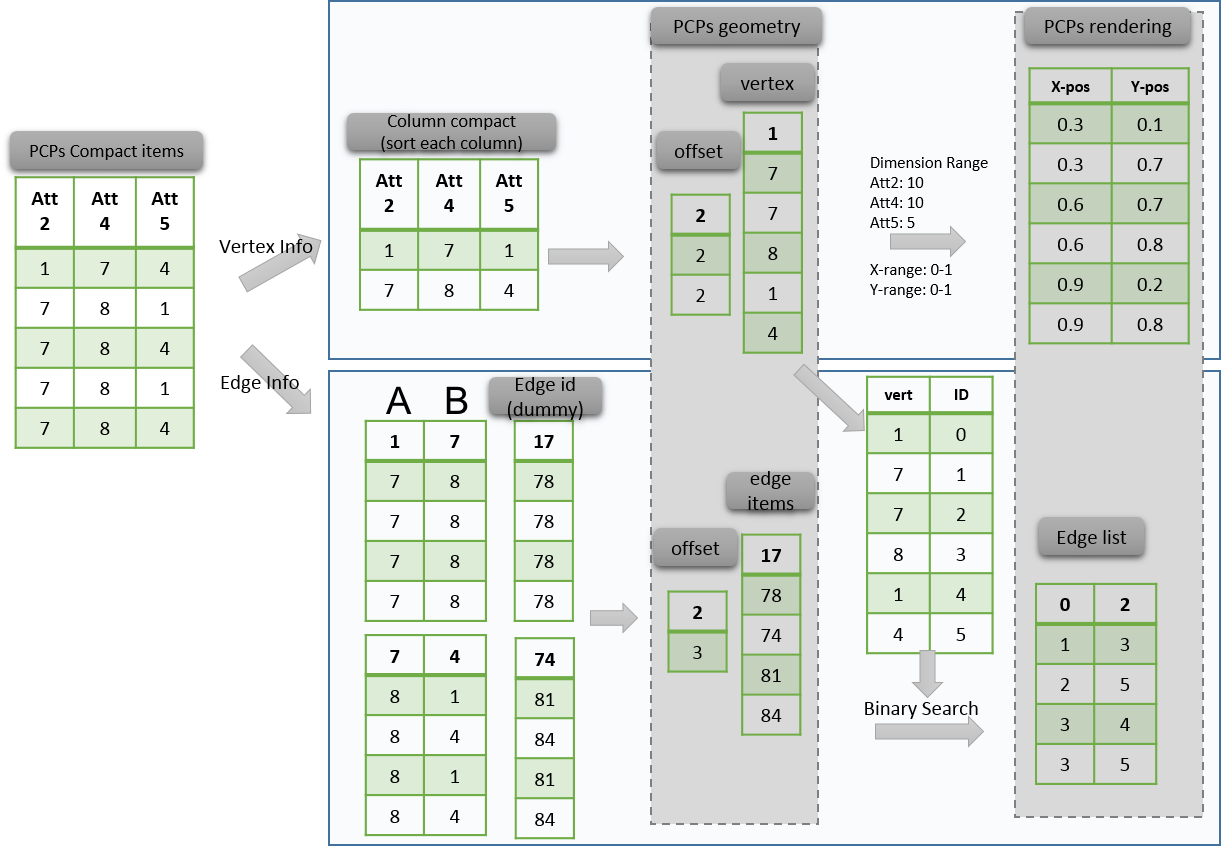
\includegraphics[width=1.0\linewidth]{pic/dataTran2.png}
	\parbox[t]{1.0\columnwidth}{\relax
	}
	%
	\caption{\label{fig:dataTran2} This figure shows data transformations from compact item lists to rendering data in parallel coordinate views. The data transformations are separated into two parts: vertex and edge data generation.}
\end{figure} 

Figure~\ref{fig:dataTran1} demonstrates data transformation from raw data into visual primitives of histogram and dynamic views. Firstly, the time window filter is applied to slice the raw data into current chunk of data. Secondly, each data record in current frame is validated by exclusive and negative exclusive filters in parallel, then they are compacted into a filtered dataset. Based on user's chosen dimension in histogram view, we group the corresponding column data to generate geometry data and transform it to rendering data based on the meta-data (data range). The data of dynamic view is straightforward. GPUs summarize the filtered data items as geometry data, then transform it to height value based on previous maximum value.

Data transformations in parallel coordinate views are more complex than other views. Firstly, GPUs generate PCPs compact items based on user chosen axes. Then the data flow is separated into two branches for generating vertex and edge data. To generate vertexes information, \textsl{unique} operator is applied to each column and then all unique values are organized into \textit{vertex} array and \textit{offset} array. Then the data ranges are applied to geometry data to obtain each node's position.
For edges, every two neighboring columns are combined into an array by their dummy values, then they are compacted and organized into \textit{edge} array and \textit{offset} array.  After this, the dummy values are unpacked, which are separated into two columns for representing edge list. At last, we replace  each vertex ID with its order ID in edge list as the rendering data.  


%\subsection{Filtering on the GPU}
%The implementation of time windows filter is straightforward, and we apply binary search of the raw data to obtain the start and end records within the time window (The raw data is stored chronologically). We generate a boolean vector, and examine each records by the exclusive filter and negative exclusive filter. Then we compact the boolean vector and 
%\subsection{Data View on the GPU}
%The dynamic view and histogram view is simple, and we focus on the parallel coordinate generation on the GPU.
%The input data is the filtered or highlighted filtered data, and the output is the edge list and node position.
%We use shader to generate the stack view and quad.

\begin{figure}[htb]
	\centering
	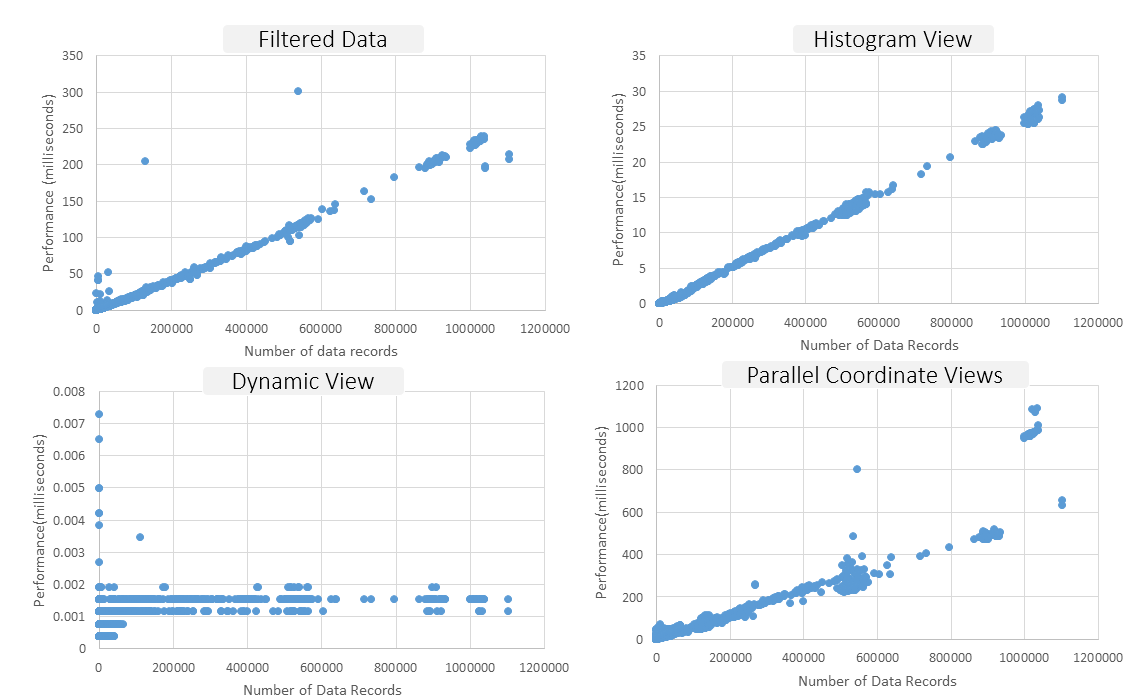
\includegraphics[width=1.0\linewidth]{pic/perf.png}
	\parbox[t]{1.0\columnwidth}{\relax
	}
	%
	\caption{\label{fig:performance}
		The performance of AVIST (without incremental computing). The scatter plots show the relationship between number of queried data records and the performance (milliseconds). From the top left to the bottom right are the performances of filtered data, histogram view, dynamic view and parallel coordinate views (four axes).  }
\end{figure}


\begin{figure*}[htb]
	\centering
	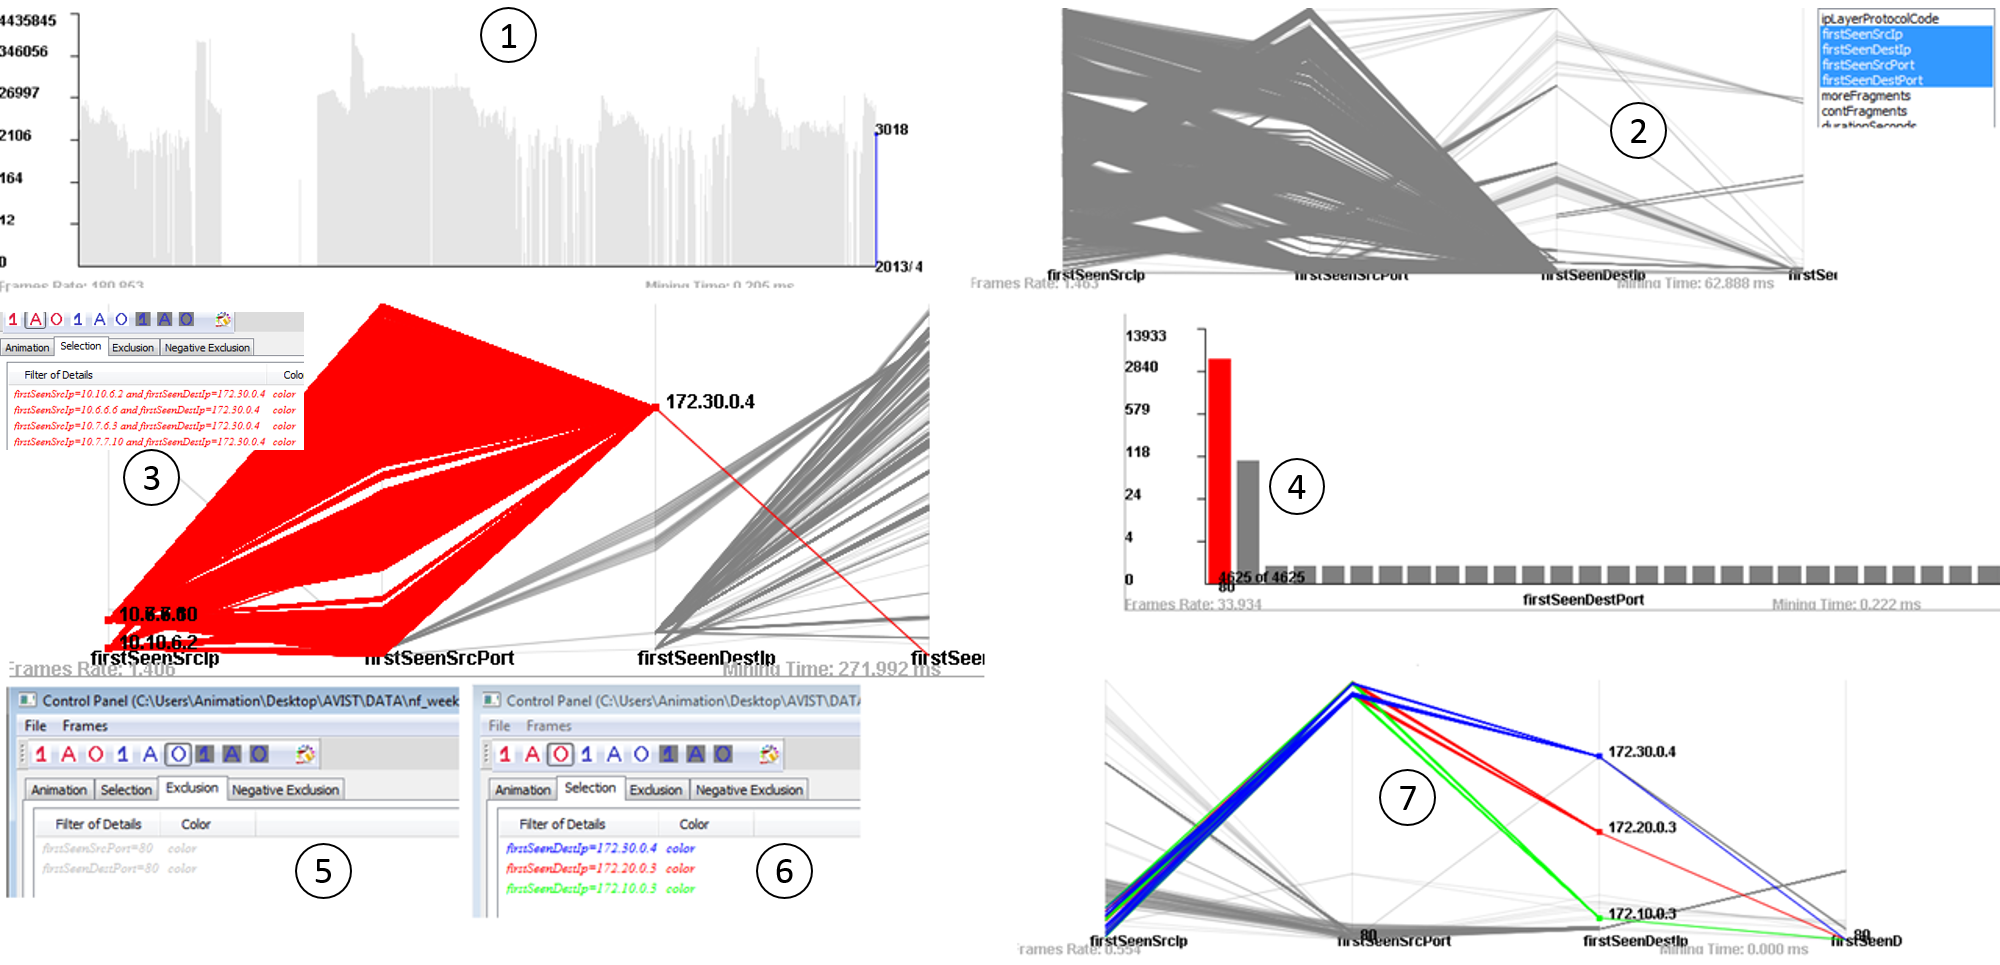
\includegraphics[width=0.9\linewidth]{pic/network2.png}
	\parbox[t]{1.0\columnwidth}{\relax
	}
	%
	\caption{\label{fig:vast}
		This figure shows a usage scenario how AVIST helps analysts to visual explore the large network logs. 
		Seven steps are presented in this figure, and Section 6.1 gives more detailed discussions for each step. }
\end{figure*}

\subsection{Performance}
%The AVIST system is written in C++ and CUDA 5.5. The visualization codes are based on OpenGL and GLSL. The interface controls are coded using wxWidgets.

We test the performance of AVIST on a desktop computer, running Windows 7 Enterprise with Service Pack 1, which is equipped with an Intel i7 processor and an NVIDIA GeForce GTX 680 graphics card with 4GB memory. We use the network traffic dataset from case study one as the benchmark.  



Based on the dependency graph design, we character  AVIST from two stages. The first stage is about filtered data generation. This stage is shared by all data views. The second stage is about each data view visual primitives generation, and their performance are independent with each other. Figure \ref{fig:performance} shows the performance in scatter plots. 
We see there is a linear relationship between the performance and the queried data records beside dynamic view.
Actually, the aggregated information in dynamic view can be easily derived by filtered dataset. The performance of parallel coordinate view is the bottleneck of AVIST. In the plot, we see that if the number of queried records exceeds 600,000, AVIST can not afford real time animation and interaction due to the hardware computation limitation. This also suggests that a user should filter more data in current time window or shrink the time window  for drilling down data details.







%\begin{figure*}[htb]
%	\centering
%	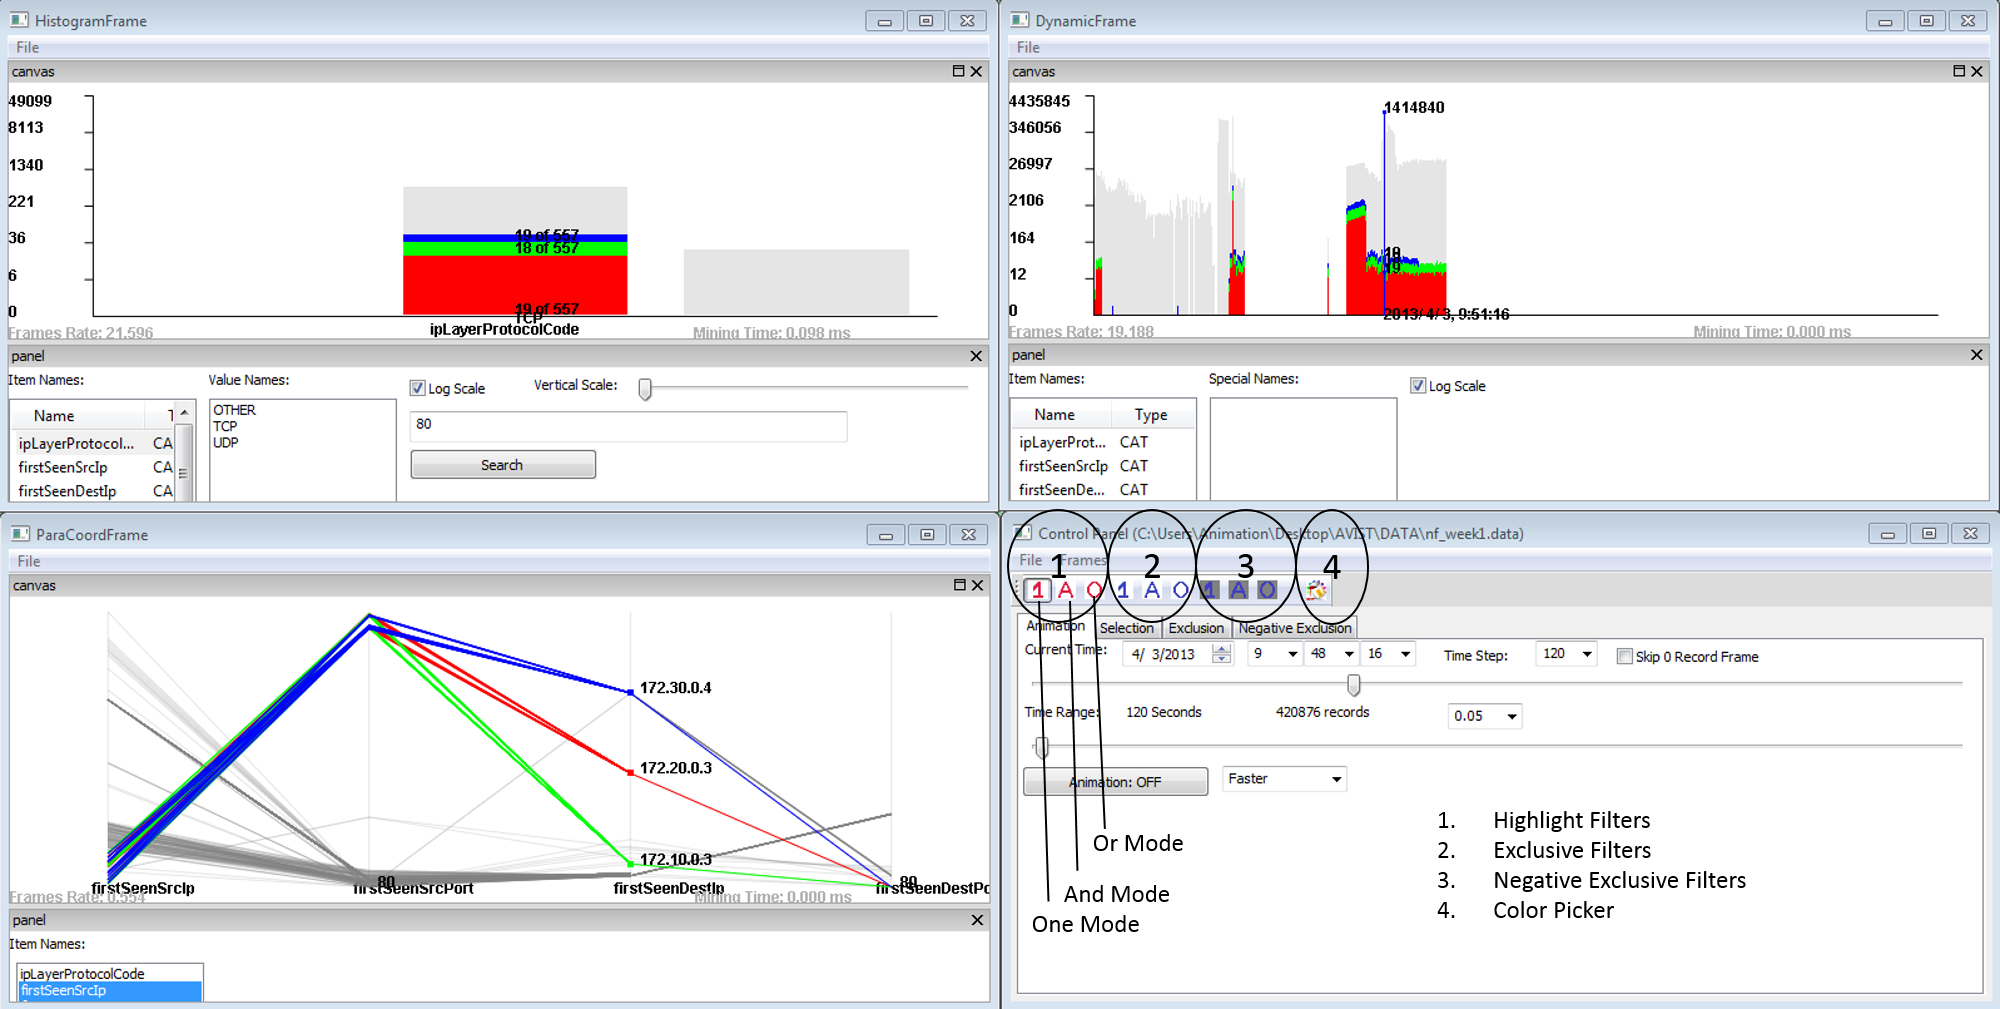
\includegraphics[width=0.8\linewidth]{pic/DataView.png}
%	\parbox[t]{1.0\columnwidth}{\relax
%	}
	%
%	\caption{\label{fig:views}
%		Three data views and control panel of AVIST. The top left is histogram view, top right is dynamic view, bottom left is parallel coordinated view and bottom right is control panel. Each data view is separated into two parts: the canvas for rendering visual primitives and the panel for exploring different data dimensions.}
%\end{figure*}  

